\subsection{Basics of Computational Neuroscience}

\label{sec:neurons_synapses}

\subsubsection{The Neuron}

The most important component of our nervous system are neurons. They are able to encode sensory input from our environment into neural representations, process the retrieved information and decode it back into behavioural output, such as movements. Neurons are the fundamental element underlying the intelligent behaviour of virtually every animal, allowing them to interact with their environment, optimize survival etc... It is widely accepted that the number of neurons within a brain correlates with a specie's intelligence, somewhat similarly to a computer which becomes more powerful with higher number of \textit{transistors}.. Figure \ref{fig:schematic_neuron} shows the schematic of a typical neuron.\\

\begin{figure}
    \centering
    \includegraphics[width=\linewidth]{Figures/neuron_schematic.png}
    \caption{Schematic of a neuron. Adapted from the lecture notes of ETH Course: "Introduction to Neuroinformatics".}
    \label{fig:schematic_neuron}
\end{figure}

There are 4 main components to the neuron: the \textbf{soma}, the \textbf{dendrites}, the \textbf{axon} and the \textbf{synapes} (not shown on figure, but we're getting there). These elements are enabling the individual neuron to connect to neighbouring neurons from which they can receive information, through synapses and dendrites, process this information, in the Soma and Synapses and propagate back information to other neurons, through axons. Intelligent behaviour is made possible by setting the connections between different neurons and the "decision" rule to send a message accordingly. There exists many different subtypes of neurons, though they all exhibit relatively similar architecture and function. 

Much of Neuroscience's research today is to understand the precise mechanisms by which neurons communicate and wire with each other. Though there are many perspectives one could focus one in order to study these dynamics, one particular paradigm of research has emerged in the recent years: \textbf{Computational Neuroscience}. This subranch of Neuroscience devotes great effort to create \textit{computational models} of brain function by modelling, often with complex mathematical equations, the behaviour of specific synpatic processes, individual neuron behaviour, and the dynamics of network of neurons. This has mainly been enabled by the rise of computing power and the improvement of imaging/recording technologies, which allowed observation, analysis and modelling of the fine dynamics exhibited in our brains. Though one particular scientific breakthrough gave birth this computational perspective: Hodgkin and Huxley's description of the \textbf{Conductance-Based Model} and the \textbf{Action Potential}.

\subsubsection{Electrical Perspective of the cell}

Hodgkin Huxley's conductance-based model \footnote{I recommend this excellent blogpost explaining the dynamics in more details: https://www.scientifica.uk.com/learning-zone/understanding-the-cell-as-an-electrical-circuit} is essentially an electrochemical model of the biological cell (the neuron is a special biological cell). 

\begin{figure}
    \centering
    \includegraphics[width=\linewidth]{Figures/Conductance_Cell.PNG}
    \caption{A) Biological cell lipid membrane, with the ion channels represented. Conductance based model of the biological cell. Adapted from the lecture notes of ETH Course: "Introduction to Neuroinformatics".}
    \label{fig:Conductance_Cell}
\end{figure}

As you know from high school biology, a cell (and also a neuron) has an intracellular body and a membrane which separates it to the extracellular space. The cell membrane consists of a double lipid layer that separates ions in the extracellular space from ions and charged proteins in the cytoplasm - it somewhat acts like an insulator. It so happens that both the intracellular space and extra cellular space are full of \textit{ions}, mainly \textit{potassium}, \textit{calcium} and \textit{sodium} ions. These ions are charged particles, and generate some electrical behaviour that we can analyze through the lense of electronic circuits. We can thus also speak of membrane voltage $V_m$, as the potential difference between the charged ions inside and outside the cell. We should also note that the cell can be seen as a \textbf{capacitor}, as it contains charged particles on both ends of an insulating layer. The insulating layer, actually contains specific \textbf{ion channels} that allow for specific ions to enter or exit the cell at specific moments. Therefore, to change the membrane voltage, it is necessary to charge the capacitance. The applied charge ($Q$) divided by the membrane capacitance ($C_m$) gives the membrane voltage ($V_m$): $V_m = Q /C_m$. We can see that for a given amount of applied charge, the smaller the membrane capacitance, the larger the membrane voltage change.

You can clearly see this on figure \ref{fig:Conductance_Cell}.A. Think of it like a dance club bouncer, allowing selected guests only to enter (or exit). Bouncer are less selective on Tuesday nights than Saturday nights: their resistance or \textbf{conductance} changes depending on the context. These basic structural components of the cell (and neuron) underlie the conductance based model that you can see on \ref{fig:Conductance_Cell}.B. We can see from the figure a few key components: 
\begin{itemize}
    \item Membrane Capacitance $C_m$: This is the capacitance that the insulating membrane carries by separating between the intracellular and extracellular space.
     \item The intracellular and extracelullar space. Flow of ions (yielding current) must go through the different channels with specific conductance levels in order to enter or exit the cell. 
    \item At rest (resting potential) the Sodium ions are in greater concentration outside the cell, and potassium ions inside the cell. This is represented with the potential levels $E_{NA}$ and $E_{K}$ configuration. 
    \item A leak current $I_L$ as the membrane is not a perfect insulator. 
\end{itemize}

All biological cells communicate with each other via electrochemical signals, which means flow of ions entering and exiting the cells in precise fashion. This is very convenient because we can apply much of our existing electronics mathematical modeling to describe these behaviours! Now that we understand and have the intuition behind the language that cells communicate with, we should understand the principal messaging characteristic: Action Potential

\subsubsection{The Action Potential}

The neuron in its neutral state, i.e. when it's not receiving or sending any messages, has a negative potential compared to its surroundings. This potential is called the \textbf{resting potential} and it's about -70 mV. It is caused by different concentrations of ions in the intracellular and the extracellular space. The "messages" a neuron receives are sudden influx or ions from neighbouring cells. These are first processed at the synapse level and eventually transmitted to the Soma through the dendrites. These can either increase the neuron's resting potential, in which case they are \textit{excitatory} input signals, or further decrease it and are \textit{inhibitory} inputs. When a neuron's potential is increased so much that it becomes larger than its a specific \textbf{threshold voltage}, it sends out a message along its axon. This message is called an \ref{fig:action_potential} (AP) and its typical course is visualized in figure \ref{fig:action_potential}. 

\begin{figure}
    \centering
    \includegraphics[width=1\linewidth]{Figures/Action_Potential_In_Full.PNG}
    \caption{A) Action Potential Voltage change through time. B) Typical course of an action potential.}
    \label{fig:action_potential}
\end{figure}

As can be seen from figure \ref{fig:action_potential}.A, once a neuron's potential crosses its threshold value, it experiences a large and fast increase of potential up to +40 mV compared to the extracellular space. This phase is called \textbf{depolarization} as the potential difference between the cell's intra- and extracellular space initially decreases. In the second phase, called the \textbf{repolarization}, the neuron's potential quickly decreases again. However, it doesn't stop at its initial resting potential but becomes even more negatively charged. This is called the hyperpolarization phase and it is denoted as refractory period in the figure. The \textbf{refractory period} is the time it takes for the neuron's potential to return back to its initial state and during this time it is not possible, or at least a lot more difficult, to generate another action potential. The action potential is commonly called a \textit{spike} and a neuron is said to fire when it generates a spike. The threshold voltage of a neuron is usually around -55 mV.\\

The idea of threshold voltage makes sense on a practical perspective: as there are \textit{many} neurons, which constantly receive inputs from everywhere, either through noise or irrelevant signaling. You want neurons to select only the strong input messages, the ones that are somewhat unusual - you want neurons to filter out the noise. Functioning with a threshold voltage is a very clever way biology figured out to implement filtering! Of course, there are very complex dynamics behind this, and the way this precisely encodes information at the scale of the network is still an active domain of research. Though a critical part of this was understood through the research of Hubel and Wiesel and Donald  Hebb, which we'll briefly touch upon in the next chapter. Essentially, you should remember two things: 1) Neurons that fire together wire together; 2) Specific neurons fire A LOT when they receive specific inputs they're sensitive to, and barely fire when these inputs are not received.

On another note, the AP can, in some sense, be considered a "digital" element \footnote{Digital, or boolean, logic is the fundamental concept underpinning all modern computer systems. Put simply, it's the system of rules that allow us to make extremely complicated decisions based on the aggregate of relatively simple 0s and 1s ("yes/no") elements. Neurons firing can be seen as 1s, and not firing as 0s.} as it either \textit{fires} when voltage goes past the threshold - or doesn't fire if voltage stats below threhsold. Whether neural computation is digital or analog is an important discussion in Neuroscience, and generally there is agreement over the fact that it is a mix of both - but that's a topic of discussion on its own. 

Now that we have looked at generation of action potentials, how can we communicate it to adjacent neurons? The generated spike travels along the axon until it reaches the axon terminals - much like an electrical signal travels through a cable. Individual neurons are not directly connected with one another but separated by the extracellular space. In order to communicate a spike across this space, we need specialized structures right at the zone of contact between neurons: the synpases. 

\subsubsection{The synapse}

In 1897 Charles Sherrington introduced the term synapse to describe the specialized structure at
the zone of contact between neurons as the point in which one neuron communicates with another.
The topic of synapses is a complex one: most of the computation of neurons actually happen at the level of the synapse. The synapse essentially is the element of the neuron that does most of the processing, and enables (or not) the action potential to happen. Synapses can be electrical or chemical, and allow excitatory or inhibitory dynamic into the post-synaptic neuron. The post synaptic neuron is simply the neuron that comes after the synapse - so if you have neuron \#1 sending message to neuron \#2, the neuron \#2 is the post synaptic one, and \#1 is the pre-synaptic one.   

\begin{figure}
    \centering
    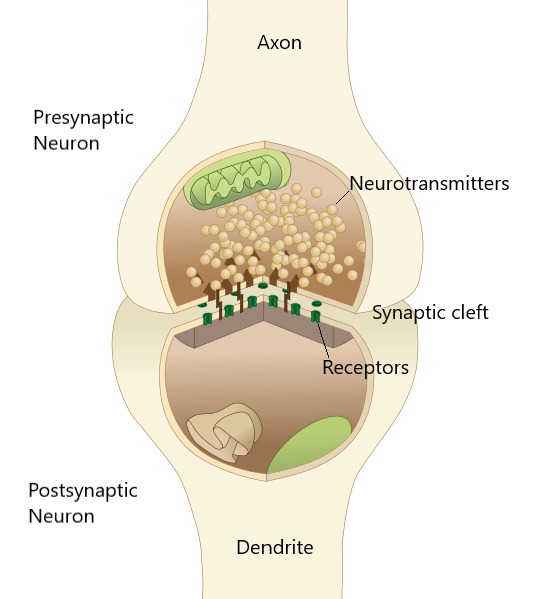
\includegraphics[width=0.8\linewidth]{Figures/Synapse.png}
    \caption{Schematic of a synapse. Adapted from Wikipedia.}
    \label{fig:synapse}
\end{figure}

As shown in the figure above, the presynaptic neuron, i.e. the axon on the top, and the postsynaptic neuron, i.e. the dendrite, are separated by extracellular space, the synaptic cleft. The presynaptic neuron is filled with chemical neurotransmitters. Once an action potential arrives at the axon, these neurotransmitters are released into the synaptic cleft. The neurotransmitters fuse across the synaptic cleft and bind to the receptors of the postsynaptic neuron. This reaction causes a depolarization or a hyperpolarization of the postsynaptic dendrite. Whether the postsynaptic neuron is de- or hyperpolarized depends on the type of the synapse and some neurotransmitter dynamics. Synpases can either be excitatory, i.e. causing a depolarizaion, or inhibitory, i.e. causing a hyperpolarization, depending on the neurotransmitters they release upon activation.\\

A biologically-plausible model of synaptic transmission is given by the alpha function. It closely matches the shape of postsynaptic potentials that were measured during in vitro experiments. The alpha function is characterized by a gradual rise followed by a slow decay. For a single incoming spike, the response of the membrane potential is defined as $u(t) = te^{-\tau t}$. $\tau$ is the synapse's decay rate which scales the output in amplitude and time. The amplitude is also shaped by the synaptic weight. Figure \ref{fig:alpha_function} visualizes the alpha function for different weights and decay rates.

\begin{figure}
 \centering
 \includegraphics[width=.6\linewidth]{Figures/alpha_function.PNG}
 \caption{Alpha function as a biologically-plausible model of synaptic transmission (Taken from \cite{comsa_temporal_2020}).}
 \label{fig:alpha_function}
\end{figure}


What is important to remember is that chemical synaptic transmission is characterized by specific temporal dynamics directly correlate to the presynaptic neuron, as shown in figure \ref{fig:Synapse_EPSP}.

\begin{figure}
    \centering
    \includegraphics[width=0.5\linewidth]{Figures/Synapse_EPSP.PNG}
    \caption{Excitatory post-synaptic potential (EPSP) in response to multiple pre-synaptic spikes. Adapted from Wikipedia.}
    \label{fig:Synapse_EPSP}
\end{figure}

Notice how the Excitatory post-synaptic potential (EPSP) changes in magnitude with the AP incoming from the pre synaptic neuron. 


% MORE CLARIFICATIONS NEEDED FROM HERE: 

% The typical synaptic input can be approximated by an alpha function of the following form:

% \begin{equation}
%     g_{syn}(t) = g_{peak} \cdot t \cdot e^{\frac{-t}{t_{peak}}}
% \end{equation}

% The function is also shown in figure \ref{fig:alpha_waveform}.

% \begin{figure}
%     \centering
%     \includegraphics[width=.6\linewidth]{Figures/alpha_waveform_synapse.PNG}
%     \caption{Alpha function that approximates synaptic input.}
%     \label{fig:alpha_waveform}
% \end{figure}

\subsubsection{Network and Computation}

One can easily see that these models of biological elements, though vastly oversimplified in my explanations, underlie very complex and intricate dynamics. In the brain, the complexity is several orders of magnitude higher, as all these elements interact with each other in a chaotic yet incredibly precise manner, which yields our ability to function. It is without surprise that many scientists chose to solely focus on understanding the emerging function from complex networks of the brain, and use the most basic of models of the brain's individual components. This simple idea has actually led to revolutionary progress, in various subfields. Mainly, Artificial Intelligence, with the Neural Network revolution. The concept is very simple: build a computational neural network, where neurons communicate with each other with a certain strength (synaptic weight for excitatory or inhibitory activation), and propagate the signal further along the network. These extremely basic models of brain function are today revolutionizing the world. Other researchers have focused on trying to replicate models of neural networks on hardware, or in less obvious fashion than in traditional machine learning. This was the purpose of the \textit{Human Brain Project} for instance, which fell short of so many of its ambitions. Carver Mead, the godfather of the field of Neuromorphic Engineering, envisionned copying some of the neural circuitry we understand in order to build faster and more efficient devices than the traditional computing counterparts. This has somewhat been successful, with the creation of the Silicon Retina by Misha Mahowald in the 1980s. 
Today, our understanding of the brain grows in complexity every day, and the idea of an elegant, simple and unified theory of neural intelligence seems more and more out of reach for humans. Nevertheless, simplified models have proven extremely effective for multiple real world applications, and it is worth looking at some of its basic concepts. It also is particularly relevant to Neuromorphic Engineering, as we will understand in due time. 